\chapter{Smart Railway Communication System}
\label{chapter2}

There has recently been growing interest in high speed railway (HSR) communication systems. This growing demand in HSR communication has led to significant activity with respect to next generation wireless communication systems applied to railway environments. Current GSM-railway (GSM-R) technology is not sufficient for satisfying the demand for large data rate applications and quality-of-service (QoS) requirements, which has subsequently led to development of Long Term Evolution for railways (LTE-R)~\cite{7553613}. LTE-R is based on the LTE architecture~\cite{7553613} and has been championed as the future of the smart railway communication systems. LTE-R provides a more efficient network architecture compared to GSM and has a reduced packet delay. It is also based on a well-established and off-the shelf communication system that provides standardized interworking mechanisms and compatibility with GSM-R. In the following sections, we discuss positive train control (PTC), wireless broadband (WiBro), train-to-train (T2T), and train-to-ground (T2G) communication, Long Term Evolution for Railways (LTE-R) communication system, spectrum regulation for railway communication systems, LTE-R services for railways, and leaky coaxial cable (LCX), all of which are important technologies for achieving smart railway transportation system.

\section{Positive Train Control}
Positive Train Control (PTC) is designed for the monitoring and controling of train movements in order to provide advanced safety operations with the help of modern wireless communication technology. The key idea behind PTC is the constant flow of information to the train about its location as well as warning engineers about train speeds in order to prevent derailment~\cite{nytimes}. Managing track occupancies through centralized route and interlocking logic, enforcing permanent and temporary speed limits for the train, and real-time localization of the train are some of the basic features implemented in PTC. 

\begin{figure}[!ht]
\centering
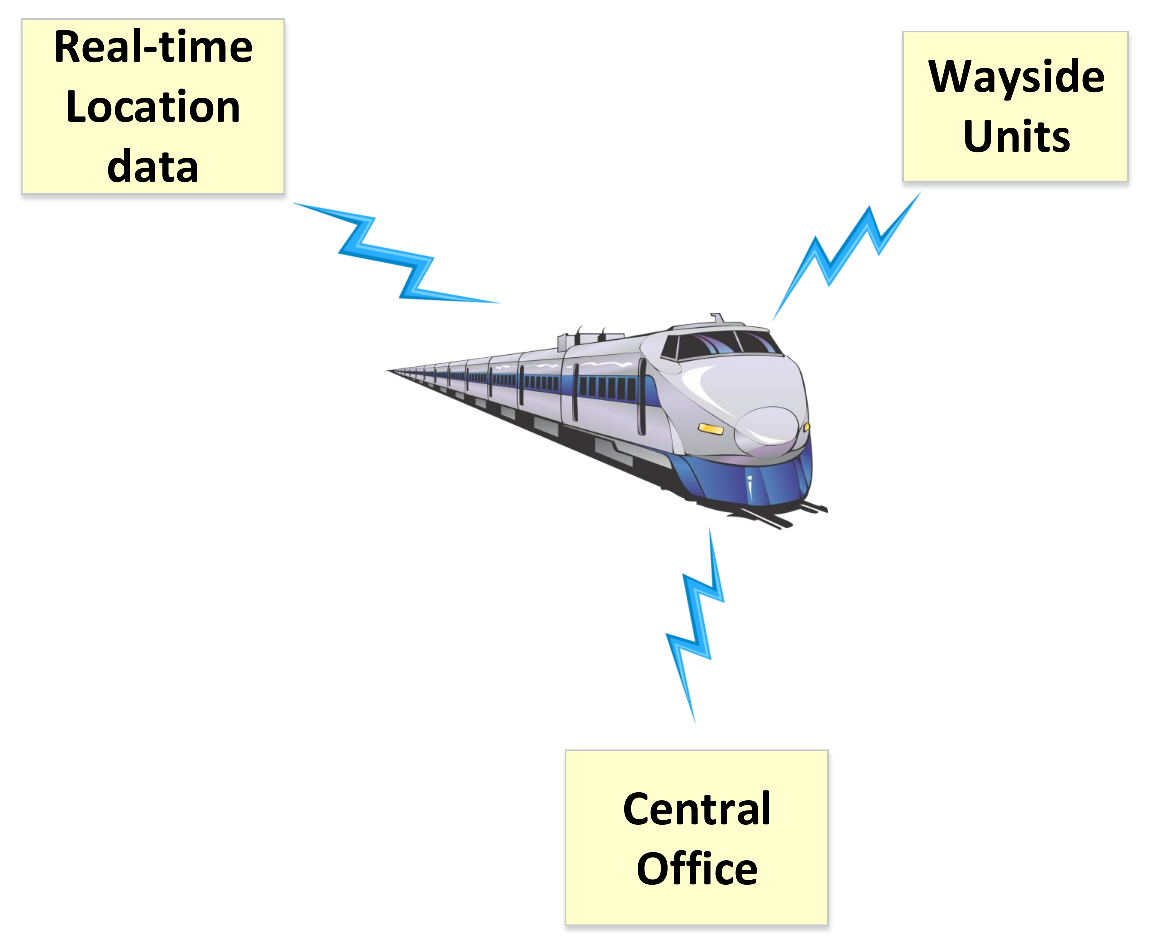
\includegraphics[width=\textwidth,height=10cm,keepaspectratio]{images/Gill/5G/ptc.eps} 
\caption{Architecture of Positive Train Control consisting of wayside units, central office and real-time GPS information. All these technologies assist PTC in achieving advance control and safety of the trains.}
\label{ptc}
\end{figure}


Figure~\ref{ptc} provides a generalized viewpoint of the PTC architecture; where the train receives the flow of information through various systems using wireless communication links. The primary means of determining location for the train is by using differential GPS, which can continuously compare its position with the stored position of speed restriction and work zones~\cite{5338992}. The Central Office (CO) regularly monitors trains, exchanging information with train management computers (TMC), and gathering precise speed and position information. The CO also collects information regarding train orders, number of cars, weight, route and track characteristics along the route, including speed restrictions, curves, grades and crossing. All wayside equipment are continuously monitored by PTC, where they issue alerts in cases when an automatic crossing gate is not working or a hot box detector senses several axles slightly above a certain temperature level. It also applies corrective action in cases where there are reports of a possible track breakage due to extreme heat or a flood.

\section{Wireless Broadband (WiBro)}

Wireless Broadband (WiBro) is a mobile broadband wireless access (BWA) service which had its first public demonstration in December 2005 and has been in service in South Korea since June 2006. WiBro was developed as a mobile BWA solution in Korea and was based on the IEEE 802.11e WiMax standard~\cite{wibro}. It is a subset of the consolidated version of the IEEE Standard 802.16-2004 (fixed wireless specifications), P802.16e (enhancements to support mobility), and P802.16-2004/Cor1 (corrections to IEEE Standard 802.16-2004). The profiles and test specifications of WiBro have been harmonized with the WiMAX Forum's mobile WiMAX profiles and test specification, resulting in a convergence of the two standards.


\begin{figure}[!ht]
\centering
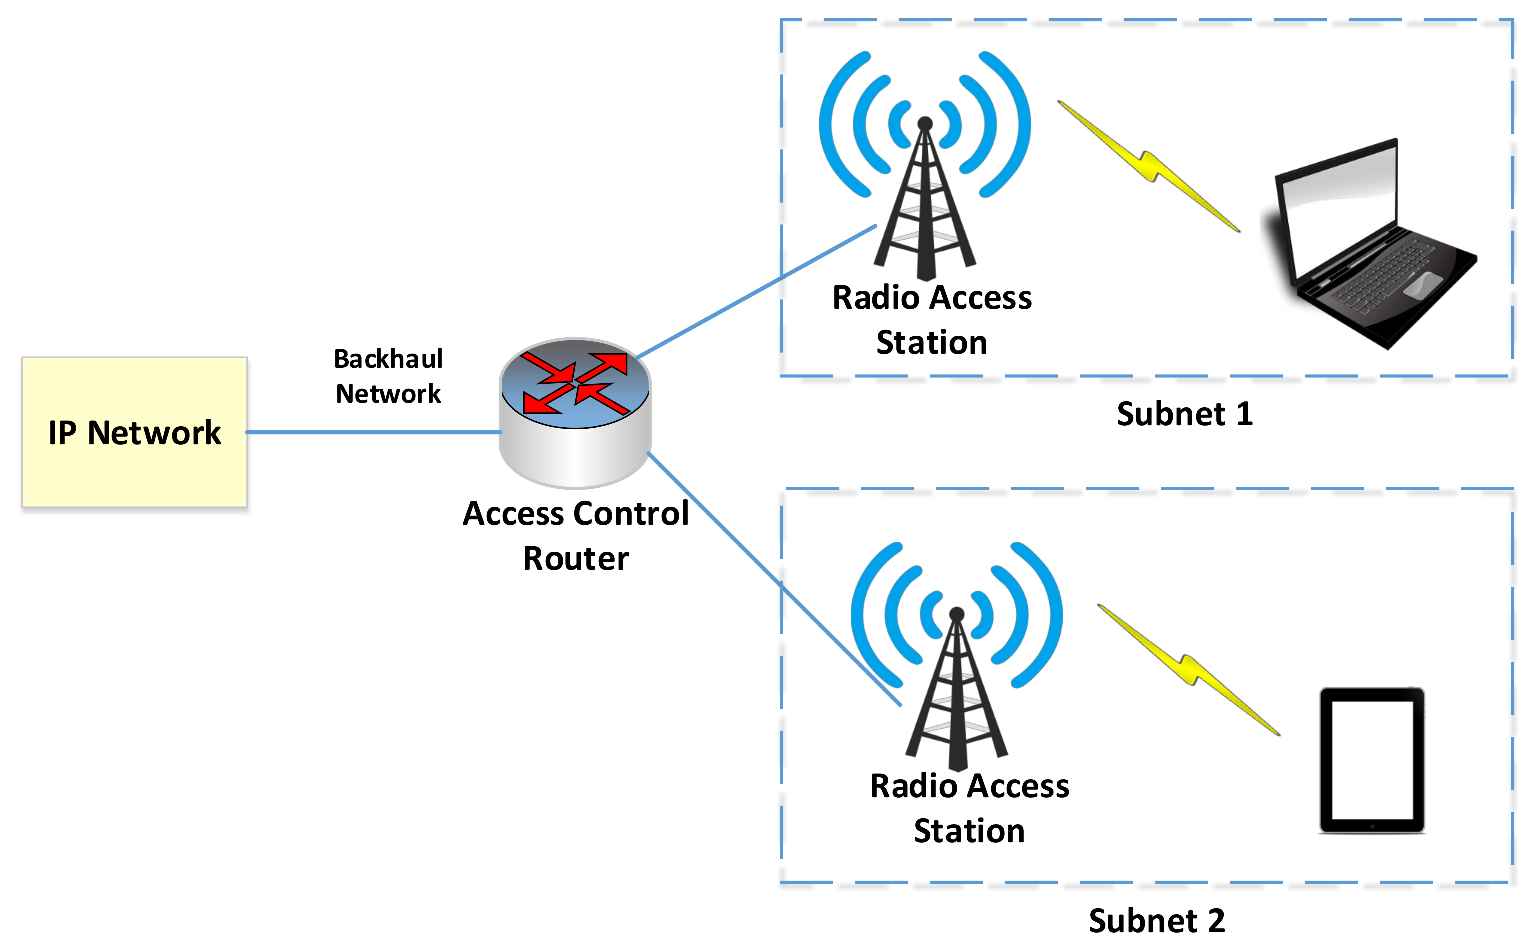
\includegraphics[width=\textwidth,height=10cm,keepaspectratio]{images/Gill/5G/wibro.eps} 
\caption{Korean Wireless Broadband (WiBro) system architecture for high speed internet connectivity. WiBro is an all IP-based network, which uses ACRs to connect the backbone network with radio access station.}
\label{wibro}
\end{figure}

Figure~\ref{wibro} describes the architecture of BWA-based WiBro communication system in the Phase I standardization~\cite{wibro}. The WiBro network consists of Access Control Routers (ACR), which connects the backbone network with a Radio Access Station (RAS). The RAS is the interface between the mobile nodes and the core network at the physical layer, and it controls the radio resources at the data link layer in conjunction with an ACR. The key distinction of WiBro from conventional cellular networks is that the Internet Protocol (IP) is used between an ACR and RASs, as well as between ACRs. WiBro uses Time Division Duplexing (TDD) or Frequency Division Duplexing (FDD) for duplexing and Orthogonal Frequency Division Multiple Access (OFDMA) for robustness against fast fading and narrow-band co-channel interference.


\section{LTE-R Communication System}

The development of a reliable wireless network for high speed trains is not a simple task and it is still an emerging technology. Global System for Mobile Communication for Railways (GSM-R)~\cite{trlter1} was a wireless communications standard designed for high speed trains, but it turned out not to be reliable enough and possessed several limitations. The data rates for voice services, which can reach up to 9.6 kbps, was unable to meet the increasing demands of high-rate data transmission for railways communication. Furthermore, the limited data rate and quality of service (QoS) requirements were not sufficient to support cellular communications. Subsequently, LTE~\cite{trlter2} proposed a promising solution for achieving broadband data rates, flexible bandwidth allocation, and high spectral efficiency in high speed trains that can overcome various GSM-R limitations~\cite{arlter3,inplter4}.

\begin{figure}[!ht]
\centering
\includegraphics[width=\textwidth,keepaspectratio]{images/Gill/lte_figs/lter_architecture.eps} 
\caption{Proposed LTE-R Architecture for next generation High-speed Railways consisting of EPA and E-UTRAN.}
\label{ltearch}
\end{figure}

LTE-R is a high speed communication standard based on the existing LTE system architecture~\cite{inplter4}. There has been several studies regarding the assessment of LTE-R as a viable choice for next generation high speed communications for railway applications~\cite{inplter5,inplter6}. Conventional LTE includes an Evolved Packet Core (EPC) network and a radio access network referred to as an Evolved Universal  Terrestrial  Radio  Access  Network (E-UTRAN). The  Internet  Protocol (IP)-based  EPC  supports  seamless handovers for both voice and data to cell towers, and each E-UTRAN cell will support high data and voice capacity by high-speed  packet  access  (HSPA).  As  a  candidate for the next-generation  communication  system  of  HSR,  LTE-R  inherits all the important features of LTE and provides an extra radio access system to exchange wireless signals with onboard  units (OBUs)  and to match HST-specific  needs. Figure~\ref{ltearch} shows the proposed architecture of LTE-R according to~\cite{trlter2}, which shows the core network of LTE-R is backward compatible with GSM-R. The network architecture of LTE-R is similar to that of LTE/SAE, with  Evolved Universal Terrestrial Radio Access Network (E-UTRAN) being the access network structure of LTE-R. The Evolved-Node B (eNodeB) units communicate directly with UEs in a similar fashion to a base transceiver station (BTS) in GSM networks. It performs the transmission and reception of data packets using Orthogonal Frequency Division Multiplexing Access (OFDMA) for downlink and Single Carrier Frequency Division Multiple Access (SC-FDMA) for uplink across the PHY layer. At the same time, as without the base-station controller (BSC), it also has radio  resource  control and wireless  mobility  management functions.  The eNodeB units can be connected to the network router directly without additional intermediate control nodes, such as the BSC in GSM-R~\cite{tingting2010high}. The main difference between EPC and the core network of GSM-R is that the EPC is an all-IP mobile core network.

\begin{table}[h!]
\caption{Comparison of system parameters between GSM-R , LTE and LTE-R.}
\begin{adjustbox}{width=\textwidth, center=\textwidth}
\begin{tabular}{| c | c | c | c |}
\toprule
System Parameters & GSM-R & LTE & LTE-R\\ 
\midrule
Frequency & \shortstack{Uplink: 876--880 MHz\\downlink: 921--925 MHz} & 800, 1800, 2600 MHz & 450, 800, 1400, 1800 MHz \\  
Capacity  & 0.2 MHz & 1.4-20 MHz & 1.4-20 MHz\\ 
Modulation  & GMSK & QPSK/16-QAM/64-QAM & QPSK/16-QAM\\ 
MIMO  & No  & 2x2, 4x4  & 2x2\\ 
Cell Range  & 8 Km  & 1-5 Km & 4-12 Km \\ 
Data Rates (DL/UL)  & 172/172 Kbps  & 100/50 Mbps & 50/10 Mbps\\ 
\bottomrule
\end{tabular}
\end{adjustbox}
\label{ltertable}
\end{table}

Conventional LTE networks are different compared to LTE-R in several ways, such as architecture, system parameters, network layout, services, and quality of service (QoS). Table~\ref{ltertable} summarizes the LTE-R parameters and describes the differences between LTE, GSM-R, and LTE-R. Since the LTE-R environment possesses very severe fading and high Doppler shift, it is configured for QoS rather than higher data rates. Therefore, QPSK modulation is used for most sub-carriers, and the number of packet re-transmissions must be kept low, which is achieved with the User Datagram Protocol (UDP).


\section{Spectrum Regulation for LTE-R}

Departing from the technical issues for a moment, we will now discuss the important interactions that smart railways will encounter with respect to spectrum policy and allocation defined by the Federal Communications Commission (FCC). The spectrum allocated for cellular technologies is already saturated in peak markets due to massive amounts of wireless services and networks. Figure~\ref{specalloc} illustrates the issue of potential spectrum scarcity in the wireless cellular bands using the frequency allocation chart of the United States~\cite{fcc}. Frequencies located at the lower portion of the spectrum can be used for wide coverage, mobility support, and control signaling while the higher portion of frequencies can be used for high data rate applications. This requires a new approach to spectrum policy and allocation methods for smart railway standardization.

\begin{figure}[!ht]
	\centering
\includegraphics[width=\textwidth,keepaspectratio]{images/Gill/5G/specalloc.eps}
	\caption{Federal Communications Commission (FCC) spectrum allocation chart~\cite{fcc}.}
	\label{specalloc}
\end{figure}

Cognitive radio is a promising technology that can solve the spectrum shortage problem resulting from the rapid increase in wireless networks and mobile devices. Recent advancements in software-defined radio technology and edge computing have enabled new Cognitive Radio Network (CRN)  capabilities and, along with some adjustments in its operation, will be a key technology for LTE-R heterogeneous network deployment. Cognitive Radio using software defined radio technology is considered to be one of the key technologies for improving the utilization of congested radio spectrum~\cite{rusek2013scaling}. Integrating CR technology into an LTE-R system is motivated by the fact that a large portion of the radio spectrum is underutilized most of the time~\cite{7553613}. For achieving data rates on order of gigabits per second, we need to make efficient use of the available spectrum, which can be achieved by using CRNs. CRNs are a secondary wireless access system that can share frequency bands with the incumbent primary wireless access system, either on an interference-free basis or an interference-tolerant basis. The CRN should be aware of
the surrounding radio environment and be capable of regulating its transmission accordingly. For interference-free CRNs, CR users are allowed to borrow spectral resources only when licensed users do not use them. The key for enabling interference-free CRNs is figuring out how to detect the spectrum holes (white spaces) that are located across the spectrum and enable dynamic spectrum access (DSA)~\cite{wyglinski2009cognitive}.

CR receivers should first monitor and allocate the unused spectrum via spectrum sensing (energy detection (ED), covariance absolute value (CAV) detection, etc.)~\cite{wyglinski2009cognitive} or by combining spectrum usage from geolocation databases and feed this information back to the central CR controller. A coordinating mechanism is required for multiple CRNs where they all try to access the same spectrum in order to prevent users colliding with each other while accessing the same spectrum holes. For interference-tolerant CRNs, CR users can share the spectrum resources with a licensed system while keeping the interference below a threshold. In comparison with interference-free CRNs, interference-tolerant CRNs can achieve enhanced spectrum utilization by opportunistically sharing the radio spectrum resources with licensed users, and can also achieve better spectral and energy efficiency. However, it has been shown that the performance of CR systems can be very sensitive to any slight change in user density, interference threshold, and transmission behavior of the licensed system~\cite{haykin2005cognitive}. However, the spectral efficiency can be improved by either relaxing the interference threshold of the primary system or considering only the CR users having short distances to the secondary BS (utilizing the spatial gain). Hybrid CRNs have been proposed in~\cite{hong2010capacity} for adoption in cellular networks in order to explore additional bands and expand the capacity. CRNs can only prove beneficial if the spectrum policies related to LTE-R are implemented in a robust manner. 

\section{Train-to-train (T2T) Railway Communication}

The development of driverless cars has imposed several strict requirements for the safety of passengers and pedestrians. For safety-critical applications, transmission delays need to be less than 10 ms, which is required for intelligent transportation systems (ITS) and vehicular networks~\cite{ge2016vehicular}. While communications for road traffic has been well investigated, with the first standards being defined for smart vehicles (ITS-G5), railway communications have mainly focused on train-to-ground (T2G) communication using GSM-R and LTE-R. Nevertheless, there are still several challenges involved in train-to-train (T2T) communications for frequencies above 1 GHz and high speed operations (up to 500 Km/h), which can potentially lead to severe fading. In~\cite{nterhuber2017wide}, a measurement campaign was performed focusing on wagon-to-wagon measurements (intra-consist) with one high speed train (HST), as well as T2T measurements with two HSTs. A survey of channel measurements and models are presented in~\cite{unterhuber2016survey}. Various simulation and experimental results revealed a trade-off between the proposed performance metrics and system parameters, such as base station (BS) and vehicle densities, radio coverage, and  the  maximum number of hops in a path. With LTE communication technologies being integrated into vehicular networks, the interference will cut down the performance of LTE vehicular networks. When vehicle density is high, the beaconing signals of the vehicular safety applications may easily overload the responsible eNodeB. To handle this issue, these signals should be handled directly between vehicles without  having to go through  the  eNB. In  LTE-Advanced (LTE-A), device-to-device (D2D) communications is considered, where direct message delivery between terminals in proximity to each other is permitted in order to decrease the load of the eNB~\cite{mumtaz2014direct}. 

\begin{figure}[!ht]
	\centering
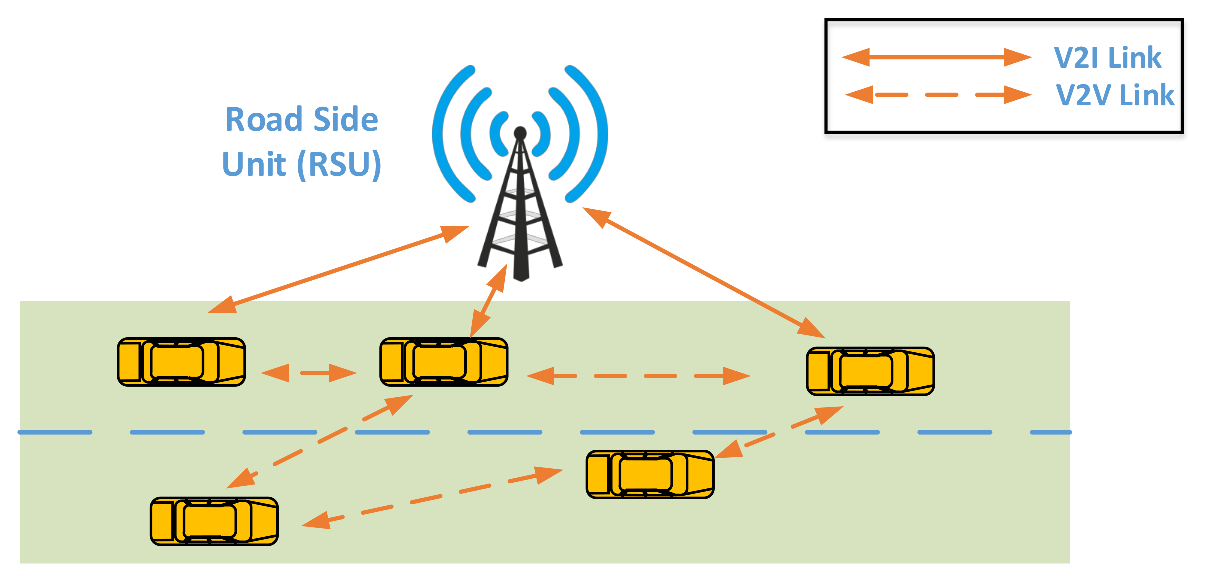
\includegraphics[width=\textwidth,keepaspectratio]{images/Gill/5G/vehiclecomm.eps}
	\caption{Vehicular communication using D2D 5G cellular communication technology.}
	\label{vcomm}
\end{figure}

The infrastructure-aided D2D technologies can serve as a natural approach for enabling reliable and efficient T2T communications without negatively affecting existing cellular systems. To meet the expected performance requirements, such as low transmission delay and high throughput, a new architecture for LTE-R vehicular communication is required. Figure~\ref{vcomm} illustrates how railway communications using the D2D strategy can offload the computation from remote road side units (RRU) to the trains in order to increase spectral efficiency. The communication environment in T2T is different than in D2D due to the high mobility (Doppler shift) of the high speed trains. Network connectivity plays a important role in T2T communication relative to D2D when comparing system throughput. These features can significantly affect D2D resource allocation strategies and system parameters, and thus should be modified for railway communication.

\section{LTE-R Services}
LTE-R provides services to improve security, quality of service (QoS), and efficiency for high speed railways. Several key services include the following:

%\begin{figure}[!ht]
%	\centering
%\includegraphics[width=\textwidth,keepaspectratio]{images/Gill/5G/device2device.eps}
%	\caption{Key LTE-R services required to augment railway security, QoS and efficiency}
%	\label{d2d}
%\end{figure}

\begin{itemize}
\item \textit{Train Control}: Train control (TC) continually monitors trains, exchanges information with Train Management Computers (TMC), and gathers precise speed and position information. TC will have a copy of train orders, number of cars, weight, route and track characteristics along the route, including speed restrictions, curves, grades and crossings. Track authority, \textit{i.e.}, permission to occupy and move on a sector of track, is continuously updated as train control computers issue or modify train orders.

\item \textit{Real-time monitoring}: LTE-R should provide video monitoring of railway track conditions (flaw detection and temperature), as well as railway infrastructure, in order to avoid accidents. The information should be transmitted in real-time with both central controller and HST with minimum delay possible. 

\item \textit{Railway Emergency Communications}: Whenever there is any natural calamity or an emergency situation, an establishment of immediate communications between accident site and rescue center is of the utmost importance. Railway emergency communications systems use railway private networks to ensure rapid deployment and faster responses compared to the existing technologies such as GSM-R. 

\item \textit{Real-time Localization for Trains}: LTE-R should be able to relay the real-time localization information to the central controller such that the efficiency of scheduling trains can be improved. With accurate localization information, train collisions can be avoided and better overall service can be provided to the passengers.

\item \textit{Railway IoT}: With railway Internet-of-Things (IoT), LTE-R can provide services such as real-time query and tracking of trains and goods. It helps to improve the transport efficiency and extend service range. Railway IoT can also help in augmenting the railway safety features.
\end{itemize}

\section{Leaky Coaxial Cable for LTE-R}
Leaky Coaxial Cable (LCX)~\cite{n1974leaky} is an antenna technology designed to deliver radio services in tunnel environment. It consists of small periodic slots to allow radio frequency (RF) signals to escape, which act as extended antenna elements. LCX cables were invented to provide the uniform signal coverage in underground mines where radio coverage can potentially be very limited due to the mine environment~\cite{arlter10}. Recently, leaky coaxial cables have been widely used in the field of railway communication, especially in tunnels~\cite{arlter10}. Leaky feeders are
constructed from coaxial cable, where the outer shield has a series of holes with different shapes and different distances amongst them. The coaxial cable is usually on the order of hundreds of metres long, and it can be installed throughout a building or a tunnel. So far, LCX have been only used to supplement wireless communication systems between a BS and trains, mostly transmitting voice signals. LCX are being used as an alternative solution to distributed antenna systems in indoor environments such as commercial buildings~\cite{motley1983directed,saleh1987distributed} and university buildings, high speed trains, and cars. The LCX radio system is almost noise free and has enough bandwidth to support multiple RF signals carrying voice and data simultaneously. Figure~\ref{fig:leakcoax} shows the conventional leaky coaxial cable along $x$-axis with periodic radiating slots and wave propagation along $z$-axis. Generally, it consists of three parts: Inner conductor, Dielectric material, and inner conductor. LCX has a dual functionality \textit{i.e.}, they can transmit and receive RF signals using their slots. The frequency range for a leaky cable is given by~\cite{cao1999radio}:
\begin{equation}
\dfrac{c}{\sqrt{\varepsilon_r-1)}d}\geq f \leq \dfrac{c}{\sqrt{\varepsilon_r}+1)d}.
\end{equation}
where $c$ is the speed of light in $m/s$, $d$ is the length of the LCX cable, and $\varepsilon_r$ is the relative permittivity of the tunnel walls.
\begin{figure}[!ht]
\centering
\includegraphics[width=\textwidth,keepaspectratio]{images/Gill/lte_figs/leakycoax.eps} 
\caption{Leaky Coaxial Cable used for uniform radio coverage in a Tunnel environment~\cite{arlter10}.}
\label{fig:leakcoax}
\end{figure}

A radio system based on LCX has been deployed in Japan for high speed railways ''Series N700''~\cite{takatsu2007history} to connect the train to the ground network. Wi-Fi access points are chosen for in-train communications with peak data rates of 2 Mbps for uplink and downlink. Although current technologies can provide wireless communication services in HSTs, the capacity of communication system is very low (1--4 Mbps). These data rates are insufficient for next generation wireless communication system where the peak data rates of 0.5 -- 5 Gbps are expected. LTE-R communication system can be implemented for achieving high data rates but it cannot be achieved by using conventional cellular systems. The penetration loss due to the tunnel walls is very high and secondly, the fast moving trains cause large Doppler shifts leading to poor connectivity due to retransmissions. Hence, leaky coaxial cable is potentially the best candidate for achieving extensive internet access inside a tunnel environment for high speed railways.

\section{Summary}
This chapter outlined and examined the topics of positive train control, WiBro, LTE-R communication system and provided a foundation for smart railway communication system. We also discuss the spectrum regulation for LTE-R, T2T railway communication, various services required in LTE-R and finally leaky coaxial cables (LCX) for uniform coverage in a tunnel environment. Next in this thesis, we consider heterogeneous cooperative spectrum sensing (CSS) and how it can be use to augment smart railways. After CSS, we discuss the implementation and results of our proposed test-bed for high speed train and software-defined radios.\\
